\chapter{Métodos e Ferramentas para Análise de Investimentos}
\label{cap:13}

\noindent\tagAV{AV2 (20\%)}\ \tagQuant
\vspace{6pt}

\begin{capObjetivos}
Ao concluir este capítulo, você será capaz de:
\begin{enumerate}[leftmargin=1.4em, itemsep=2pt]
  \item Aplicar o princípio do valor do dinheiro no tempo por meio de juros compostos, desconto intertemporal e definição da Taxa Mínima de Atratividade (\textbf{TMA}) como custo de oportunidade.
  \item Construir passo a passo o \textbf{Fluxo de Caixa Livre (FCL)} a partir de receitas, OPEX, depreciação, imposto de renda, variação de capital de giro e CAPEX.
  \item Calcular, interpretar e decidir com base nos principais indicadores de viabilidade: \textbf{VPL}, \textbf{TIR} (reconhecendo múltiplas TIRs e a hipótese de reinvestimento), \textbf{MTIR}, \textbf{VAUE} (para projetos com vidas úteis distintas), \textbf{Payback Simples} e \textbf{Payback Descontado}.
  \item Conduzir análises de sensibilidade e cenários (otimista, base e pessimista) para avaliar a robustez de projetos tecnológicos e territoriais.
\end{enumerate}
\end{capObjetivos}

\begin{capRevisao}
Antes de modelar os fluxos descontados, retome três conceitos do Capítulo 12:
\begin{itemize}[leftmargin=1.4em, itemsep=2pt]
  \item \textbf{CAPEX versus OPEX:} o investimento fixo ocorre no Ano $0$ (ou em expansões pontuais) e é recuperado economicamente ao longo da vida útil, enquanto o OPEX se repete a cada período operacional.
  \item \textbf{Capital de Giro ($NLCG$):} variações positivas na necessidade de giro consomem caixa no período em que ocorrem e são recuperadas ao final do horizonte do projeto.
  \item \textbf{Limitação do Ponto de Equilíbrio:} o equilíbrio contábil anual não incorpora o custo de oportunidade do capital imobilizado nem a distribuição dos fluxos ao longo dos anos.
\end{itemize}
\end{capRevisao}

\etapa{3}{Valor do Dinheiro no Tempo, Fluxo de Caixa Livre e Indicadores}

\subsection{Valor do dinheiro no tempo e Taxa Mínima de Atratividade (TMA)}

Um real recebido hoje vale mais do que um real a ser recebido daqui a um ano por três razões objetivas: \textbf{custo de oportunidade} (o capital disponível hoje pode render juros em aplicações alternativas), \textbf{inflação} (perda de poder de compra) e \textbf{risco} (incerteza quanto ao recebimento futuro). No regime de juros compostos, um Valor Presente ($VP$) capitalizado à taxa $i$ por $t$ períodos gera um Valor Futuro $VF = VP \cdot (1 + i)^t$; inversamente, trazer um fluxo futuro $FC_t$ para a data zero exige dividi-lo pelo fator $(1 + TMA)^t$.

A \textbf{Taxa Mínima de Atratividade (TMA)} é a taxa de retorno mínima que o investidor ou empreendedor exige para aceitar o projeto, equivalente ao rendimento da melhor alternativa disponível de risco comparável (custo de oportunidade do capital).

\begin{boxSimbolo}[Vocabulário Conceitual e Símbolos do Capítulo 13]
Na modelagem intertemporal, $FC_t$ ou $FCL_t$ indica o Fluxo de Caixa Livre no período $t$ ($t = 0, 1, \dots, n$), descontado pela Taxa Mínima de Atratividade ($TMA$, expressa em decimal, como $0{,}12$ para $12\%$ a.a.). A criação absoluta de riqueza em moeda presente é medida pelo Valor Presente Líquido ($VPL$, em \reais{}), complementado pelo Índice de Lucratividade ($IL$).

Entre os indicadores de taxa e prazo, $TIR$ designa a Taxa Interna de Retorno que anula o VPL, enquanto $MTIR$ representa a Taxa Interna de Retorno Modificada, calculada com taxa de financiamento $k_f$ e taxa de reinvestimento $k_r$. Por meio do Fator de Recuperação de Capital $FRC(i,n)$, o Valor Anual Uniforme Equivalente ($VAUE$) permite comparar alternativas de durações distintas. O tempo de recuperação do capital é aferido pelo Payback Simples ($PBS$) e pelo Payback Descontado ($PBD$, em anos ou períodos), ao passo que a apuração do fluxo parte do Lucro Antes do Imposto de Renda ($LAIR$), da Depreciação contábil ($Depr$) e da Variação de Capital de Giro ($\Delta CG$).
\end{boxSimbolo}

\subsection{Construção do Fluxo de Caixa Livre (FCL)}

A análise de investimentos utiliza \textbf{caixa efetivo}, nunca apenas lucro contábil. Como a depreciação reduz o lucro tributável sem representar saída de dinheiro do caixa, ela é subtraída para calcular o imposto de renda e somada de volta após o imposto.

\begin{boxFormula}[Estrutura Padrão do Fluxo de Caixa Livre ($FCL_t$)]
\begin{align*}
  \text{LAIR}_t &= \text{Receita}_t - \text{OPEX}_{\text{desembolsável}, t} - \text{Depreciação}_t \\
  \text{Lucro Líquido}_t &= \text{LAIR}_t \times (1 - T_{\text{IR/CSLL}}) \\
  \text{FCO}_t &= \text{Lucro Líquido}_t + \text{Depreciação}_t \\
  \text{FCL}_t &= \text{FCO}_t - \Delta \text{CG}_t - \text{CAPEX}_t + \text{Valor Residual líquido}_t
\end{align*}
No Ano $0$, geralmente $\text{FCL}_0 = -\text{CAPEX}_0 - \text{CG}_0$. Ao final do horizonte $n$, o capital de giro acumulado é recuperado ($\Delta \text{CG}_n < 0$, somando caixa).
\end{boxFormula}

\subsection{Métodos de Análise de Investimentos}

\begin{boxFormula}[VPL, TIR, MTIR, VAUE e Payback]
\textbf{1. Valor Presente Líquido (VPL):} origem na matemática financeira de Irving Fisher (1930); mede a riqueza líquida absoluta criada pelo projeto em moeda de hoje.
\[
  VPL = \sum_{t=0}^{n} \frac{FCL_t}{(1 + TMA)^t} = FCL_0 + \frac{FCL_1}{(1+TMA)^1} + \dots + \frac{FCL_n}{(1+TMA)^n}
\]
\textit{Critério de decisão:} aceitar se $VPL > 0$; rejeitar se $VPL < 0$; indiferente se $VPL = 0$. Entre projetos mutuamente excludentes de mesma duração, escolher o de maior $VPL$. O Índice de Lucratividade complementar é $IL = \frac{\sum_{t=1}^{n} FCL_t/(1+TMA)^t}{|FCL_0|}$ (aceitar se $IL > 1$).

\vspace{5pt}
\textbf{2. Taxa Interna de Retorno (TIR):} taxa de desconto $r^*$ que iguala o VPL a zero:
\[
  \sum_{t=0}^{n} \frac{FCL_t}{(1 + TIR)^t} = 0
\]
\textit{Critério de decisão:} para projetos convencionais (um sinal negativo em $t=0$ seguido de positivos), aceitar se $TIR > TMA$. Dois problemas críticos limitam esse indicador. Em fluxos não convencionais, com múltiplas inversões de sinal (como descomissionamento ambiental no último ano), a equação polinomial gera \textbf{múltiplas TIRs} ou nenhuma raiz real (Regra dos Sinais de Descartes); além disso, a TIR pressupõe implicitamente que os fluxos intermediários positivos são reinvestidos à própria $TIR$, o que é irrealista quando a $TIR$ é muito superior à taxa de mercado.

\vspace{5pt}
\textbf{3. Taxa Interna de Retorno Modificada (MTIR):} corrige o pressuposto irrealista de reinvestimento da TIR descontando os fluxos negativos à taxa de financiamento ($k_f$) até $t=0$ e capitalizando os fluxos positivos à taxa de reinvestimento ($k_r$, geralmente a $TMA$) até $t=n$:
\[
  MTIR = \left( \frac{\sum_{t: FCL_t > 0} FCL_t (1 + k_r)^{n-t}}{\sum_{t: FCL_t < 0} \frac{|FCL_t|}{(1 + k_f)^t}} \right)^{\frac{1}{n}} - 1
\]
\textit{Critério de decisão:} aceitar se $MTIR > TMA$. Garante solução única mesmo com múltiplos fluxos negativos.

\vspace{5pt}
\textbf{4. Valor Anual Uniforme Equivalente (VAUE):} indispensável para comparar projetos mutuamente excludentes com \textbf{vidas úteis diferentes} ($n_A \neq n_B$), pois converte o VPL total em uma série uniforme anual equivalente:
\[
  VAUE = VPL \times FRC(TMA, n), \qquad \text{onde} \quad FRC(i, n) = \frac{i(1+i)^n}{(1+i)^n - 1}
\]
\textit{Critério de decisão:} entre alternativas de durações distintas com possibilidade de renovação, escolher o projeto de maior $VAUE$ positivo.

\vspace{5pt}
\textbf{5. Payback Simples ($PBS$) e Payback Descontado ($PBD$):} medem o tempo necessário para recuperar o investimento inicial. O $PBS$ soma fluxos nominais (ignorando o valor do dinheiro no tempo); o $PBD$ soma os fluxos já trazidos a valor presente pela $TMA$. Se a recuperação ocorrer entre os anos $k$ e $k+1$:
\[
  PBD = k + \frac{|\text{Saldo Descontado Acumulado}_{k}|}{VP(FCL_{k+1})}
\]
\end{boxFormula}

A Figura~\ref{fig:13_perfil} ilustra o comportamento do Valor Presente Líquido em função da taxa de desconto, evidenciando o ponto em que a curva cruza o eixo horizontal (a própria TIR) e permitindo comparar projetos mutuamente excludentes sob diferentes custos de oportunidade.

\begin{figure}[H]
  \centering
  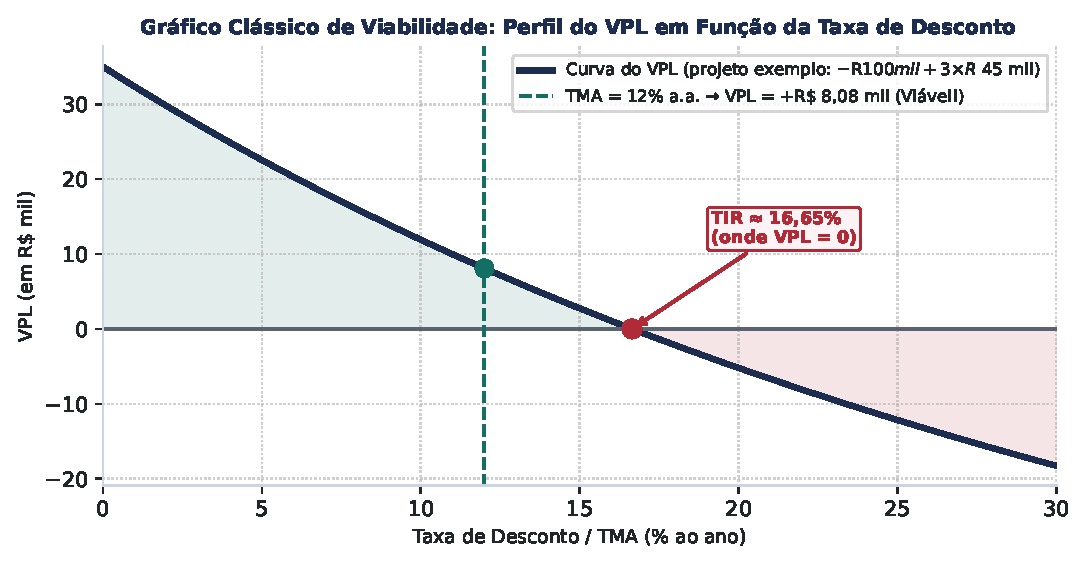
\includegraphics[width=0.88\textwidth]{figures/fig13_perfil_vpl_tir.pdf}
  \caption{Perfil do Valor Presente Líquido (VPL) em função da taxa de desconto, interseção com a TIR e comparação de projetos.}
  \label{fig:13_perfil}
\end{figure}

\subsection{Análise de sensibilidade e cenários}

Como projeções financeiras contêm incerteza quanto a preços, custos e demanda territorial, avalia-se a robustez do VPL por dois caminhos complementares. Na \textbf{Análise de Sensibilidade (univariada)}, você varia uma única premissa por vez, mantendo as demais constantes (por exemplo, preço em $-10\%$, OPEX em $+15\%$ ou $TMA$ oscilando de $8\%$ a $16\%$), para identificar qual variável exerce maior impacto sobre a viabilidade do projeto. Já na \textbf{Análise de Cenários (multivariada)}, definem-se estados macroeconômicos e territoriais consistentes (\textit{Pessimista}, \textit{Base} e \textit{Otimista}) com probabilidades atribuídas $p_s$ ($\sum p_s = 1$), calculando-se o VPL esperado pela média ponderada $\mathbb{E}[VPL] = \sum_s p_s \cdot VPL_s$.

\etapa{4}{Exemplos Resolvidos Passo a Passo}

\begin{boxExemplo}{13.1}{Construção Completa do Fluxo de Caixa Livre (FCL)}
\passoEnunciado{Uma empresa de tecnologia limpa implanta um biodigestor modular para agroindústria regional com horizonte de $3$ anos.}
\passoDados{Ano $0$: CAPEX = \reais{300.000} (depreciação linear em $3$ anos, sem valor residual) e capital de giro inicial ($CG_0$) = \reais{40.000}. Anos $1$ a $3$: Receita anual = \reais{250.000}; OPEX desembolsável anual = \reais{110.000}; alíquota de IR/CSLL = $34\%$. No Ano $1$, há reforço adicional de capital de giro ($\Delta CG_1 = +\reais{10.000}$); no Ano $2$, $\Delta CG_2 = 0$; no Ano $3$, todo o capital de giro acumulado (\reais{50.000}) é recuperado ($\Delta CG_3 = -\reais{50.000}$). $TMA = 10\%$ a.a.}
\passoPedido{Calcular o $FCL_0, FCL_1, FCL_2, FCL_3$ e o $VPL$ do projeto.}
\passoMetodo{Cálculo da depreciação anual ($300.000 / 3$), apuração do LAIR e IR/CSLL, soma da depreciação de volta para obter o FCO e ajuste pela variação de capital de giro e CAPEX.}
\passoContas{%
\begin{align*}
  \text{Depreciação anual} &= \frac{300.000}{3} = \reais{100.000/\text{ano}} \\
  \text{LAIR}_{1,2,3} &= 250.000 - 110.000 - 100.000 = \reais{40.000/\text{ano}} \\
  \text{IR/CSLL (34\%)} &= 40.000 \times 0{,}34 = \reais{13.600/\text{ano}} \\
  \text{Lucro Líquido}_{1,2,3} &= 40.000 - 13.600 = \reais{26.400/\text{ano}} \\
  \text{FCO}_{1,2,3} &= 26.400 + 100.000 = \reais{126.400/\text{ano}} \\[6pt]
  FCL_0 &= -300.000 - 40.000 = -\reais{340.000} \\
  FCL_1 &= 126.400 - 10.000 = \reais{116.400} \\
  FCL_2 &= 126.400 - 0 = \reais{126.400} \\
  FCL_3 &= 126.400 + 50.000 = \reais{176.400} \\[6pt]
  VPL &= -340.000 + \frac{116.400}{1{,}10} + \frac{126.400}{1{,}10^2} + \frac{176.400}{1{,}10^3} \\
  &= -340.000 + 105.818{,}18 + 104.462{,}81 + 132.531{,}93 = +\reais{2.812{,}92}
\end{align*}
}
\passoResposta{$FCL = [-\reais{340.000};\, \reais{116.400};\, \reais{126.400};\, \reais{176.400}]$ e $VPL = \mathbf{+\reais{2.812{,}92}}$ (projeto marginalmente viável).}
\passoVerificacao{Se o projetista esquecesse de somar a depreciação de volta ou ignorasse a recuperação dos \reais{50.000} de capital de giro no Ano $3$, o projeto pareceria inviável.}
\end{boxExemplo}

\begin{boxExemplo}{13.2}{Cálculo de VPL e Índice de Lucratividade (Energia Solar Comunitária)}
\passoEnunciado{Uma cooperativa de irrigação no Semiárido avalia instalar uma usina solar fotovoltaica compartilhada para reduzir custos de bombeamento.}
\passoDados{Investimento inicial $FCL_0 = -\reais{200.000}$. Economia líquida anual constante durante $4$ anos: $FCL_1 = FCL_2 = FCL_3 = FCL_4 = \reais{75.000/\text{ano}}$. $TMA = 12\%$ a.a.}
\passoPedido{Calcular o Valor Presente das entradas ($VP_{+}$), o $VPL$ e o Índice de Lucratividade ($IL$).}
\passoMetodo{Desconto individual de cada fluxo pela fator $(1{,}12)^t$, subtração de $|FCL_0|$ e cálculo de $IL = VP_{+} / |FCL_0|$.}
\passoContas{%
\begin{align*}
  VP_1 &= \frac{75.000}{1{,}12^1} = \frac{75.000}{1{,}12} = \reais{66.964{,}29} \\
  VP_2 &= \frac{75.000}{1{,}12^2} = \frac{75.000}{1{,}2544} = \reais{59.789{,}54} \\
  VP_3 &= \frac{75.000}{1{,}12^3} = \frac{75.000}{1{,}404928} = \reais{53.383{,}52} \\
  VP_4 &= \frac{75.000}{1{,}12^4} = \frac{75.000}{1{,}573519} = \reais{47.663{,}86} \\[4pt]
  VP_{+} &= 66.964{,}29 + 59.789{,}54 + 53.383{,}52 + 47.663{,}86 = \reais{227.801{,}20} \\
  VPL &= 227.801{,}20 - 200.000 = +\reais{27.801{,}20} \\
  IL &= \frac{227.801{,}20}{200.000} = 1{,}139
\end{align*}
}
\passoResposta{$VP_{+} = \mathbf{\reais{227.801{,}20}}$; $VPL = \mathbf{+\reais{27.801{,}20}}$; $IL = \mathbf{1{,}14}$ (projeto aprovado).}
\passoVerificacao{O $IL = 1{,}139$ mostra que cada \reais{1{,}00} investido retorna \reais{1{,}14} em valor presente já descontado à TMA de $12\%$ a.a.}
\end{boxExemplo}

\begin{boxExemplo}{13.3}{TIR por Interpolação Linear, Payback Simples e Payback Descontado}
\passoEnunciado{Uma startup de logística reversa avalia um projeto com fluxo de caixa $FCL = [-\reais{100.000};\, \reais{40.000};\, \reais{50.000};\, \reais{60.000}]$ e $TMA = 10\%$ a.a.}
\passoDados{$FCL_0 = -100.000$; $FCL_1 = 40.000$; $FCL_2 = 50.000$; $FCL_3 = 60.000$; $TMA = 10\%$ a.a.}
\passoPedido{Calcular o Payback Simples ($PBS$), o Payback Descontado ($PBD$) à $TMA = 10\%$ e estimar a $TIR$ por interpolação entre $20\%$ e $25\%$.}
\passoMetodo{Acumulação nominal para $PBS$; desconto de cada fluxo a $10\%$ e acumulação para $PBD$; cálculo de $VPL(20\%)$ e $VPL(25\%)$ seguido de interpolação linear para a $TIR$.}
\passoContas{%
\textbf{1. Payback Simples ($PBS$):} \\
Saldo Ano $0 = -100.000$; Ano $1 = -100.000 + 40.000 = -60.000$; Ano $2 = -60.000 + 50.000 = -10.000$. No Ano $3$, entram \reais{60.000}:
\[
  PBS = 2 + \frac{10.000}{60.000} = 2{,}17\text{ anos}
\]
\textbf{2. Payback Descontado ($PBD$ a $10\%$):} \\
$VP_1 = 40.000 / 1{,}10 = \reais{36.363{,}64}$ (Saldo $= -63.636{,}36$) \\
$VP_2 = 50.000 / 1{,}21 = \reais{41.322{,}31}$ (Saldo $= -22.314{,}05$) \\
$VP_3 = 60.000 / 1{,}331 = \reais{45.078{,}89}$ (Saldo $= +22.764{,}84 = VPL$)
\[
  PBD = 2 + \frac{22.314{,}05}{45.078{,}89} = 2{,}50\text{ anos}
\]
\textbf{3. Estimativa da TIR:} \\
$VPL(20\%) = -100.000 + \frac{40.000}{1{,}20} + \frac{50.000}{1{,}44} + \frac{60.000}{1{,}728} = -100.000 + 33.333{,}33 + 34.722{,}22 + 34.722{,}22 = +\reais{2.777{,}78}$ \\
$VPL(25\%) = -100.000 + \frac{40.000}{1{,}25} + \frac{50.000}{1{,}5625} + \frac{60.000}{1{,}953125} = -100.000 + 32.000 + 32.000 + 30.720 = -\reais{5.280{,}00}$
\[
  TIR \approx 20\% + 5\% \times \frac{2.777{,}78}{2.777{,}78 - (-5.280{,}00)} = 20\% + 5\% \times 0{,}3447 = 21{,}72\%\quad (\text{exata: } 21{,}65\%)
\]
}
\passoResposta{$PBS = \mathbf{2{,}17\text{ anos}}$; $PBD = \mathbf{2{,}50\text{ anos}}$; $VPL(10\%) = \mathbf{+\reais{22.764{,}84}}$; $TIR = \mathbf{21{,}65\%\text{ a.a.}}$ ($> 10\%$).}
\passoVerificacao{O $PBD$ ($2{,}50$ anos) é sempre maior que o $PBS$ ($2{,}17$ anos) quando $TMA > 0$, pois os fluxos futuros descontados valem menos em moeda de hoje.}
\end{boxExemplo}

\begin{boxExemplo}{13.4}{Comparação entre TIR e MTIR (Reinvestimento Realista)}
\passoEnunciado{Um projeto de automação agroindustrial exige \reais{120.000} em $t=0$ e gera fluxos de \reais{55.000}, \reais{65.000} e \reais{70.000} nos anos $1$, $2$ e $3$.}
\passoDados{$FCL = [-120.000;\, 55.000;\, 65.000;\, 70.000]$; taxa de financiamento $k_f = 8\%$ a.a.; taxa de reinvestimento de mercado $k_r = TMA = 12\%$ a.a.}
\passoPedido{Calcular a $MTIR$ e compará-la com a $TIR$ exata do projeto ($25{,}77\%$ a.a.).}
\passoMetodo{Capitalização de todas as entradas positivas até $t=3$ à taxa $k_r = 12\%$, manutenção da saída negativa em $t=0$ (já está na data zero) e extração da raiz cúbica.}
\passoContas{%
\begin{align*}
  VF_{+} &= 55.000 \times 1{,}12^2 + 65.000 \times 1{,}12^1 + 70.000 \\
  &= (55.000 \times 1{,}2544) + (65.000 \times 1{,}12) + 70.000 \\
  &= 68.992{,}00 + 72.800{,}00 + 70.000{,}00 = \reais{211.792{,}00} \\[4pt]
  VP_{-} &= \reais{120.000{,}00} \\[4pt]
  MTIR &= \left(\frac{211.792{,}00}{120.000{,}00}\right)^{\frac{1}{3}} - 1 = (1{,}764933)^{0{,}333333} - 1 = 1{,}2085 - 1 = 20{,}85\%\text{ a.a.}
\end{align*}
}
\passoResposta{$MTIR = \mathbf{20{,}85\%\text{ a.a.}}$ (inferior à TIR de $25{,}77\%$, mas ainda superior à TMA de $12\%$).}
\passoVerificacao{A TIR ($25{,}77\%$) superestimou a rentabilidade porque assumiu que os \reais{55.000} do Ano $1$ seriam reaplicados a $25{,}77\%$ ao ano. A MTIR ($20{,}85\%$) reflete o retorno composto real quando os saldos intermediários são reinvestidos à taxa realista de $12\%$.}
\end{boxExemplo}

\begin{boxExemplo}{13.5}{VAUE para Vidas Úteis Diferentes e Análise de Cenários}
\passoEnunciado{Uma prefeitura e um consórcio tecnológico devem escolher entre dois equipamentos mutuamente excludentes para triagem automatizada de resíduos: Equipamento $A$ (vida útil de $2$ anos) ou Equipamento $B$ (vida útil de $3$ anos), ambos renováveis e avaliados à $TMA = 10\%$ a.a. Em seguida, avalia-se a sensibilidade probabilística do projeto vencedor.}
\passoDados{Equipamento $A$: $FCL_A = [-100.000;\, 65.000;\, 65.000]$. Equipamento $B$: $FCL_B = [-140.000;\, 65.000;\, 65.000;\, 65.000]$. Para a análise de cenários de mercado do projeto, estimam-se três estados: Otimista ($p=25\%$, $VPL = \reais{80.000}$), Base ($p=50\%$, $VPL = \reais{30.000}$) e Pessimista ($p=25\%$, $VPL = -\reais{20.000}$).}
\passoPedido{Calcular $VPL_A$, $VPL_B$, $VAUE_A$ e $VAUE_B$ para decidir qual equipamento adotar; em seguida, calcular o $VPL$ esperado ($\mathbb{E}[VPL]$).}
\passoMetodo{Cálculo dos VPLs individuais, conversão para base anual via $VAUE = VPL \times \frac{i(1+i)^n}{(1+i)^n - 1}$ e média ponderada pelas probabilidades dos cenários.}
\passoContas{%
\begin{align*}
  VPL_A &= -100.000 + \frac{65.000}{1{,}10} + \frac{65.000}{1{,}21} = -100.000 + 59.090{,}91 + 53.719{,}01 = \reais{12.809{,}92} \\
  FRC(10\%, 2) &= \frac{0{,}10 \times 1{,}21}{1{,}21 - 1} = \frac{0{,}121}{0{,}21} = 0{,}576190 \\
  VAUE_A &= 12.809{,}92 \times 0{,}576190 = \reais{7.380{,}95/\text{ano}} \\[6pt]
  VPL_B &= -140.000 + \frac{65.000}{1{,}10} + \frac{65.000}{1{,}21} + \frac{65.000}{1{,}331} \\
  &= -140.000 + 59.090{,}91 + 53.719{,}01 + 48.835{,}46 = \reais{21.645{,}38} \\
  FRC(10\%, 3) &= \frac{0{,}10 \times 1{,}331}{1{,}331 - 1} = \frac{0{,}1331}{0{,}331} = 0{,}402115 \\
  VAUE_B &= 21.645{,}38 \times 0{,}402115 = \reais{8.703{,}93/\text{ano}} \\[6pt]
  \mathbb{E}[VPL] &= (0{,}25 \times 80.000) + (0{,}50 \times 30.000) + (0{,}25 \times (-20.000)) \\
  &= 20.000 + 15.000 - 5.000 = +\reais{30.000{,}00}
\end{align*}
}
\passoResposta{Deve-se escolher o \textbf{Equipamento B} ($VAUE_B = \mathbf{\reais{8.703{,}93/\text{ano}}} > VAUE_A = \reais{7.380{,}95/\text{ano}}$). O $VPL$ esperado nos cenários é \textbf{+\reais{30.000,00}}.}
\passoVerificacao{Comparar apenas os VPLs brutos ($12{,}8$ mil contra $21{,}6$ mil) seria metodologicamente incorreto porque $B$ dura $3$ anos e $A$ dura $2$ anos. O $VAUE$ coloca ambos na mesma régua anual e confirma a superioridade de $B$.}
\end{boxExemplo}

\etapa{5}{Armadilhas Conceituais e Erros Mais Comuns}

\begin{boxErro}[Erro 1: Esquecer de somar a depreciação de volta no FCL]
A depreciação não gera desembolso de caixa; ela apenas reduz o lucro tributável (benefício fiscal da depreciação). Se você subtrair a depreciação para achar o LAIR e não a somar novamente após o IR/CSLL, subestimará o fluxo de caixa do projeto.
\end{boxErro}

\begin{boxErro}[Erro 2: Usar VPL bruto para comparar projetos com vidas úteis diferentes]
Comparar o VPL de uma máquina que dura $2$ anos com o de outra que dura $5$ anos favorece artificialmente o projeto mais longo. Para horizontes distintos e renováveis, é obrigatório converter ambos em \textbf{VAUE}.
\end{boxErro}

\begin{boxErro}[Erro 3: Confiar cegamente na TIR em projetos com inversão de sinal ou escalas distintas]
Um projeto pequeno pode ter $TIR = 50\%$ e $VPL = \reais{5.000}$, enquanto um projeto maior tem $TIR = 22\%$ e $VPL = \reais{80.000}$. Além disso, fluxos com saída negativa no final geram múltiplas TIRs. Na dúvida entre projetos mutuamente excludentes de mesma duração, decida pelo \textbf{maior VPL}.
\end{boxErro}

\begin{boxErro}[Erro 4: Decidir exclusivamente pelo Payback Simples]
O Payback Simples ignora o valor do dinheiro no tempo e desconsidera todos os fluxos posteriores à data de recuperação. Projetos de infraestrutura ou P\&D que maturam nos anos $3$ a $5$ seriam injustamente descartados pelo critério exclusivo de payback curto.
\end{boxErro}

\etapa{6}{Lista de Exercícios de Fixação (15 Questões)}

\begin{enumerate}[leftmargin=1.6em, itemsep=5pt]
  \item Qual é o valor futuro de um capital de \reais{50.000} aplicado durante $3$ anos à taxa composta de $12\%$ a.a.? \espacoResolucao[1.5cm]
  \item Uma unidade produtiva projeta no Ano $1$: Receita = \reais{400.000}, OPEX desembolsável = \reais{220.000}, Depreciação = \reais{60.000}, alíquota de IR = $25\%$ e aumento de capital de giro ($\Delta CG$) = \reais{20.000} (sem CAPEX adicional no Ano $1$). Calcule o $FCL_1$. \espacoResolucao[1.8cm]
  \item Calcule o $VPL$ e o Índice de Lucratividade ($IL$) do fluxo $FCL = [-\reais{150.000};\, \reais{60.000};\, \reais{70.000};\, \reais{80.000}]$ à $TMA = 10\%$ a.a. \espacoResolucao[1.8cm]
  \item Determine a $TIR$ exata do projeto de $2$ anos com fluxo $FCL = [-\reais{100.000};\, \reais{50.000};\, \reais{84.000}]$. (Dica: resolva a equação quadrática em $x = 1 + TIR$). \espacoResolucao[1.8cm]
  \item Para o fluxo $FCL = [-\reais{90.000};\, \reais{33.000};\, \reais{48.400};\, \reais{53.240}]$ e $TMA = 10\%$ a.a., calcule o Payback Simples ($PBS$) e o Payback Descontado ($PBD$). \espacoResolucao[1.8cm]
  \item Calcule a $MTIR$ do projeto $FCL = [-\reais{100.000};\, \reais{50.000};\, \reais{50.000};\, \reais{50.000}]$, adotando taxa de financiamento $k_f = 10\%$ a.a. e taxa de reinvestimento $k_r = 10\%$ a.a. \espacoResolucao[1.8cm]
  \item Dois projetos mutuamente excludentes têm vidas úteis diferentes e serão avaliados à $TMA = 10\%$ a.a.: Projeto $X$ ($2$ anos) apresenta $VPL_X = \reais{20.000}$; Projeto $Y$ ($4$ anos) apresenta $VPL_Y = \reais{34.000}$. Calcule o $VAUE$ de cada projeto e indique qual deve ser escolhido. \espacoResolucao[1.8cm]
  \item Demonstre que o projeto não convencional $FCL = [-\reais{100.000};\, \reais{230.000};\, -\reais{132.000}]$ possui duas TIRs distintas: $10\%$ e $20\%$. Calcule o $VPL$ em ambas as taxas. \espacoResolucao[1.7cm]
  \item Em uma análise de cenários, um projeto apresenta $VPL = -\reais{30.000}$ no cenário Pessimista ($20\%$), $VPL = \reais{40.000}$ no cenário Base ($50\%$) e $VPL = \reais{100.000}$ no cenário Otimista ($30\%$). Calcule o $VPL$ esperado. \espacoResolucao[1.6cm]
  \item Avalie a sensibilidade à taxa de desconto do projeto $FCL = [-\reais{100.000};\, \reais{60.000};\, \reais{60.000}]$ calculando o $VPL$ para $TMA = 8\%$ a.a. e para $TMA = 15\%$ a.a. \espacoResolucao[1.7cm]
  \item Explique por que a hipótese de reinvestimento da TIR tradicional distorce a avaliação de projetos com retornos muito elevados (ex.: $TIR = 60\%$ a.a.) quando o mercado oferece $12\%$ a.a. \espacoResolucao[1.5cm]
  \item Qual é o impacto de um aumento na alíquota de IR/CSLL sobre o $VPL$ de um projeto e por que a depreciação funciona como escudo fiscal? \espacoResolucao[1.5cm]
  \item Quando o $VPL$ de um projeto é exatamente igual a zero, o que isso significa em termos de remuneração do investidor e relação entre $TIR$ e $TMA$? \espacoResolucao[1.5cm]
  \item Por que a recuperação do capital de giro no último ano do projeto ($t=n$) deve ser somada ao fluxo de caixa, mesmo que não gere lucro contábil? \espacoResolucao[1.5cm]
  \item Em projetos de infraestrutura hídrica ou saneamento territorial com benefícios sociais difusos e longo prazo de maturação, por que uma $TMA$ excessivamente alta tende a inviabilizar iniciativas socialmente desejáveis? \espacoResolucao[1.5cm]
\end{enumerate}

\etapa{7}{Desafios Autorais e Aplicação Territorial (Preparação AV3)}

\begin{enumerate}[leftmargin=1.6em, itemsep=5pt]
  \item \textbf{Modelagem de FCL na AV3:} Estruture os 3 primeiros anos do Fluxo de Caixa Livre do projeto do seu grupo (Receita estimada, OPEX, Depreciação, IR, $\Delta CG$ e CAPEX inicial), justificando a $TMA$ adotada com base no custo de oportunidade ou taxa do financiamento regional. \espacoResolucao[2.0cm]
  \item \textbf{Sensibilidade Territorial:} Escolha a variável mais crítica do seu projeto (preço pago ao produtor, produtividade agrícola ou tarifa de energia) e simule o impacto de uma variação adversa de $20\%$ sobre o $VPL$. \espacoResolucao[1.8cm]
  \item \textbf{Vida Útil e Tecnologia:} Compare duas alternativas tecnológicas para o seu projeto com vidas úteis distintas (por exemplo, equipamento nacional de $3$ anos versus importado de $5$ anos), explicando como o $VAUE$ resolve o impasse. \espacoResolucao[1.6cm]
\end{enumerate}

\begin{boxDica}[Contraponto Crítico e Prática Territorial (AV2 e AV3)]
Na modelagem financeira de projetos de base territorial, nunca utilize $TMA = 0\%$ nem omita o efeito do tempo. Mesmo projetos apoiados por subvenção econômica a fundo perdido (como editais FINEP/FAPESB) precisam demonstrar sustentabilidade operacional após o término do subsídio: calcule o $VPL$ considerando a reposição de equipamentos ($CAPEX$ de manutenção) e a formação de capital de giro próprio.
\end{boxDica}

\clearpage
\etapa{8}{Gabarito Integralmente Comentado (Exercícios 1 a 15 + Desafios 1 a 3)}

\begin{boxGabarito}[Resolução Passo a Passo: Exercícios de Fixação (1 a 15)]
\begin{enumerate}[leftmargin=1.5em, itemsep=4pt]
  \item \textbf{Juros compostos:} $VF = 50.000 \times (1{,}12)^3 = 50.000 \times 1{,}404928 = \mathbf{\reais{70.246{,}40}}$.
  \item \textbf{FCL Ano 1:} $LAIR = 400.000 - 220.000 - 60.000 = \reais{120.000}$. $IR(25\%) = \reais{30.000}$. Lucro Líquido $= \reais{90.000}$. $FCO = 90.000 + 60.000 = \reais{150.000}$. $FCL_1 = 150.000 - 20.000 = \mathbf{\reais{130.000}}$.
  \item \textbf{VPL e IL:} $VP_1 = 60.000/1{,}1 = 54.545{,}45$; $VP_2 = 70.000/1{,}21 = 57.851{,}24$; $VP_3 = 80.000/1{,}331 = 60.105{,}18$. $VP_{+} = \reais{172.501{,}88}$. $VPL = 172.501{,}88 - 150.000 = \mathbf{+\reais{22.501{,}88}}$. $IL = 172.501{,}88 / 150.000 = \mathbf{1{,}15}$.
  \item \textbf{TIR exata:} $-100.000 + \frac{50.000}{x} + \frac{84.000}{x^2} = 0 \Rightarrow x^2 - 0{,}5x - 0{,}84 = 0$. Discriminante $\Delta = 0{,}25 + 3{,}36 = 3{,}61 \Rightarrow \sqrt{\Delta} = 1{,}90$. Raiz positiva: $x = (0{,}5 + 1{,}90)/2 = 1{,}20 \Rightarrow TIR = \mathbf{20\%\text{ a.a.}}$.
  \item \textbf{PBS e PBD:}
  $PBS$: Ano $1$ ($33.000$, falta $57.000$); Ano $2$ ($48.400$, falta $8.600$); Ano $3$ ($53.240$) $\Rightarrow PBS = 2 + 8.600/53.240 = \mathbf{2{,}16\text{ anos}}$. \\
  $PBD(10\%)$: $VP_1 = 33.000/1{,}1 = 30.000$ (saldo $-60.000$); $VP_2 = 48.400/1{,}21 = 40.000$ (saldo $-20.000$); $VP_3 = 53.240/1{,}331 = 40.000 \Rightarrow PBD = 2 + 20.000/40.000 = \mathbf{2{,}50\text{ anos}}$.
  \item \textbf{MTIR:} $VF_{+} = 50.000(1{,}10^2 + 1{,}10^1 + 1) = 50.000(1{,}21 + 1{,}10 + 1) = 50.000 \times 3{,}31 = \reais{165.500}$. $MTIR = (165.500 / 100.000)^{1/3} - 1 = (1{,}655)^{1/3} - 1 = \mathbf{18{,}29\%\text{ a.a.}}$.
  \item \textbf{VAUE:}
  $FRC(10\%, 2) = 0{,}10 \times 1{,}21 / 0{,}21 = 0{,}576190 \Rightarrow VAUE_X = 20.000 \times 0{,}576190 = \mathbf{\reais{11.523{,}81/\text{ano}}}$. \\
  $FRC(10\%, 4) = 0{,}10 \times 1{,}4641 / 0{,}4641 = 0{,}315471 \Rightarrow VAUE_Y = 34.000 \times 0{,}315471 = \mathbf{\reais{10.726{,}01/\text{ano}}}$. \\
  Escolher \textbf{Projeto X} (maior VAUE).
  \item \textbf{Múltiplas TIRs:}
  Para $10\%$: $-100.000 + 230.000/1{,}1 - 132.000/1{,}21 = -100.000 + 209.090{,}91 - 109.090{,}91 = \mathbf{0}$. \\
  Para $20\%$: $-100.000 + 230.000/1{,}2 - 132.000/1{,}44 = -100.000 + 191.666{,}67 - 91.666{,}67 = \mathbf{0}$. Ambas anulam o VPL.
  \item \textbf{VPL Esperado:} $\mathbb{E}[VPL] = 0{,}20(-30.000) + 0{,}50(40.000) + 0{,}30(100.000) = -6.000 + 20.000 + 30.000 = \mathbf{+\reais{44.000}}$.
  \item \textbf{Sensibilidade à TMA:}
  Para $8\%$: $VPL = -100.000 + 60.000/1{,}08 + 60.000/1{,}1664 = -100.000 + 55.555{,}56 + 51.440{,}33 = \mathbf{+\reais{6.995{,}88}}$. \\
  Para $15\%$: $VPL = -100.000 + 60.000/1{,}15 + 60.000/1{,}3225 = -100.000 + 52.173{,}91 + 45.368{,}62 = \mathbf{-\reais{2.457{,}47}}$.
  \item \textbf{Reinvestimento da TIR:} A fórmula matemática da TIR assume implicitamente que cada fluxo positivo intermediário é reaplicado à própria TIR ($60\%$), o que raramente existe no mercado. A MTIR corrige isso usando a TMA ($12\%$).
  \item \textbf{IR e depreciação:} Maior alíquota de IR reduz o fluxo de caixa após impostos e diminui o VPL. A depreciação reduz o lucro tributável sem saída de caixa, gerando economia fiscal igual a $\text{Depreciação} \times T$.
  \item \textbf{VPL = 0:} O projeto remunera exatamente a TMA (custo de oportunidade), não gerando riqueza extra além do mínimo exigido; nesse ponto, $TIR = TMA$.
  \item \textbf{Recuperação de CG:} O capital de giro imobilizado em estoques e contas a receber durante a operação retorna ao caixa na liquidação do ciclo no ano final, compondo o fluxo livre disponível ao investidor.
  \item \textbf{TMA alta e longo prazo:} Taxas de desconto elevadas penalizam exponencialmente os fluxos distantes no fator $(1+TMA)^t$, tornando projetos de longa maturação inviáveis sob ótica estritamente privada de curto prazo.
\end{enumerate}
\end{boxGabarito}

\begin{boxGabarito}[Diretrizes de Resposta: Desafios Autorais (1 a 3)]
\begin{enumerate}[leftmargin=1.5em, itemsep=3pt]
  \item \textbf{Desafio 1:} O grupo deve explicitar a tabela completa Receita $\to$ OPEX $\to$ Depreciação $\to$ LAIR $\to$ IR $\to$ FCO $\to$ $\Delta CG$ $\to$ FCL, vinculando a TMA à Selic ou ao custo de captação do FNE/BNDES acrescido de prêmio de risco.
  \item \textbf{Desafio 2:} Deve recalcular o FCL após o choque de $-20\%$ na variável crítica e comparar o novo VPL com o cenário base, identificando o ponto de virada (break-even financeiro).
  \item \textbf{Desafio 3:} Deve demonstrar que o VAUE iguala os horizontes temporais distintos ao converter cada VPL em uma anuidade equivalente à TMA do projeto.
\end{enumerate}
\end{boxGabarito}

\begin{boxResumo}
\begin{itemize}[leftmargin=1.4em, itemsep=2pt]
  \item O \textbf{Fluxo de Caixa Livre} parte do lucro operacional após impostos, soma a depreciação de volta e desconta investimentos em CAPEX e variações de Capital de Giro.
  \item O \textbf{VPL} mede a criação absoluta de riqueza líquida em valor presente ($VPL > 0$ aprova o projeto).
  \item A \textbf{TIR} falha em fluxos não convencionais (múltiplas raízes) e assume reinvestimento à própria TIR; a \textbf{MTIR} resolve ambas as falhas.
  \item Projetos mutuamente excludentes com vidas úteis diferentes devem ser comparados pelo \textbf{VAUE}, nunca pelo VPL bruto.
\end{itemize}
\end{boxResumo}

\begin{boxTeste}
\begin{enumerate}[leftmargin=1.5em, itemsep=4pt]
  \item Calcule o $VPL$ do fluxo $FCL = [-\reais{80.000};\, \reais{44.000};\, \reais{48.400}]$ à $TMA = 10\%$ a.a.
  \item Calcule o Payback Descontado ($PBD$) do fluxo $FCL = [-\reais{60.000};\, \reais{22.000};\, \reais{36.300};\, \reais{26.620}]$ à $TMA = 10\%$ a.a.
  \item (\V/\F) Na comparação entre dois projetos mutuamente excludentes de $2$ e $4$ anos, o critério correto de desempate é o maior VPL bruto.
  \item (\V/\F) O Payback Descontado é sempre maior ou igual ao Payback Simples quando a $TMA > 0$ e os fluxos operacionais são positivos.
\end{enumerate}
\vspace{4pt}
\noindent\textbf{Gabarito do Checkpoint:} \textbf{1.} $VP_1 = 44.000/1{,}1 = 40.000$; $VP_2 = 48.400/1{,}21 = 40.000 \Rightarrow VPL = -80.000 + 40.000 + 40.000 = \mathbf{\reais{0{,}00}}$ ($TIR = 10\%$). \quad \textbf{2.} $VP_1 = 20.000$ (saldo $-40.000$); $VP_2 = 30.000$ (saldo $-10.000$); $VP_3 = 20.000 \Rightarrow PBD = 2 + 10.000/20.000 = \mathbf{2{,}50\text{ anos}}$. \quad \textbf{3.} \F\ (deve-se usar o VAUE). \quad \textbf{4.} \V.
\end{boxTeste}
